%
% File acl2012.tex
%
% Contact: Maggie Li (cswjli@comp.polyu.edu.hk), Michael White (mwhite@ling.osu.edu)
%%
%% Based on the style files for ACL2008 by Joakim Nivre and Noah Smith
%% and that of ACL2010 by Jing-Shin Chang and Philipp Koehn


\documentclass[11pt,a4paper]{article}
\renewcommand{\baselinestretch}{1.035}
\usepackage{acl2014}
\usepackage{times}
\usepackage{latexsym}
\usepackage{amsmath}
\usepackage{color}
\usepackage{epsfig,url,algorithm,algorithmic,multirow}
%\usepackage{microtype}
\usepackage{amssymb}


%for writing 
%\usepackage{amsfonts}
%\usepackage{amssymb}
%\usepackage{calligra}
%\usepackage{calrsfs}
%\usepackage[left=2cm,right=2cm,top=2cm,bottom=2cm]{geometry}
%\usepackage[mathscr]{euscript}


%%EXTRA HOME-GROWN MACROS

\newcommand{\tom}[1]{{\color{blue}(TOM: \textit{#1})}}
%\newcommand{\tom}[1]{{}}

\newcommand{\squishlist}{
 \begin{list}{$\bullet$}
  { \setlength{\itemsep}{0pt}
     \setlength{\parsep}{3pt}
     \setlength{\topsep}{3pt}
     \setlength{\partopsep}{0pt}
     \setlength{\leftmargin}{1.5em}
     \setlength{\labelwidth}{1em}
     \setlength{\labelsep}{0.5em} } }

\newcommand{\squishlisttwo}{
 \begin{list}{$\bullet$}
  { \setlength{\itemsep}{0pt}
     \setlength{\parsep}{0pt}
    \setlength{\topsep}{0pt}
    \setlength{\partopsep}{0pt}
    \setlength{\leftmargin}{2em}
    \setlength{\labelwidth}{1.5em}
    \setlength{\labelsep}{0.5em} } }

\newcommand{\squishend}{\end{list}}

\newtheorem{theorem}{Theorem}
\newtheorem{lemma}{Lemma}
\newtheorem{corollary}{Corollary}
\newtheorem{definition}{Definition}
\newtheorem{example}{Example}
\newtheorem{hypothesis}{Hypothesis}
%\newtheorem{hypothesis}{Hypothesis}[section]
\newcommand{\newWord}[1]{\emph{#1}}
\newcommand{\ignore}[1]{}
%\newcommand{\comment}[1]{{\color{red}{#1}}}
\newcommand{\comment}[1]{}
%\newcommand{\remark}[1]{{\color{red}{#1}}}
\newcommand{\indented}[1]{
	\begin{tabbing}
		blah\=\+\kill
		\parbox{8cm}{#1}
	\end{tabbing}
}
\renewcommand{\paragraph}[1]{\noindent\textbf{#1.}}
\newcommand{\ruleline}[1]{\indented{#1}}



\newcommand{\fact}{{\footnotesize \texttt}}
\newcommand{\factid}[2]{\emph{#1:} \texttt{#2}}
\newcommand{\factspo}[3]{{\footnotesize $<$\texttt{#1}, \texttt{#2}, \texttt{#3}$>$}}
\newcommand{\factidspo}[4]{\emph{#1:} \texttt{#2} \texttt{#3} \texttt{#4}}
\newcommand{\spotl}[1]{\texttt{<#1>}}
\newcommand{\spotlfive}[5]{$\langle$\texttt{#1}, \texttt{#2}, \texttt{#3}, [\texttt{#4}], $\mathtt{#5}\rangle$}
\newcommand{\entity}[1]{{\footnotesize \texttt{#1}}}
%\newcommand{\entity}{{\footnotesize \texttt}}
\newcommand{\rel}[1]{{\footnotesize \texttt{#1}}}

\newcommand{\instance}[1]{\textit{$\langle$#1$\rangle$}}
\newcommand{\pos}[1]{\textit{#1}}
\newcommand{\pattern}[1]{\textit{#1}}
\newcommand{\str}[1]{``#1''}
\newcommand{\svo}{\pattern{{\instance{S}}V{\instance{O}}}}


\newcommand{\unimportant}[1]{#1}
%\newcommand{\unimportant}[1]{}

\newcommand{\word}[1]{``#1''}

%%%%%%%%%%%% system
\newcommand{\sellname}{Prepper}

\newcommand{\highlight}[1]{{\color{red} #1}}

%\usepackage{acl-hlt2011}
\usepackage{times}
\usepackage{latexsym}
\usepackage{amsmath}
\usepackage{bbm}
\usepackage{multirow}
\usepackage{url}
\DeclareMathOperator*{\argmax}{arg\,max}

\usepackage{booktabs}
\usepackage{graphicx}
\usepackage{varwidth}



% take from http://tex.stackexchange.com/questions/40283/wrapping-table-column-headings-in-turn-environment
\newcommand{\turn}[3][10em]{% \turn[<width>]{<angle>}{<stuff>}
  \rlap{\rotatebox{#2}{\begin{varwidth}[t]{#1}#3\end{varwidth}}}%
}

\title{A Knowledge-Intensive Model for Prepositional Phrase Attachment}

%\title{A Knowledge-Intensive Model for\\ Extracting Information from  Prepositional Phrases}
%\tom{\\ A Knowledge-Intensive Model for Prepositional Phrase Attachment} \\
%\tom{\\ A Knowledge-Intensive Model for Reading Prepositional Phrases}}

\author{Ndapandula Nakashole \\
  Carnegie Mellon University \\
  5000 Forbes Avenue \\
  Pittsburgh, PA, 15213 \\
  {\tt ndapa@cs.cmu.edu} \\\And
  Tom M. Mitchell \\
  Carnegie Mellon University \\
  5000 Forbes Avenue \\
  Pittsburgh, PA, 15213 \\
  {\tt tom.mitchell@cs.cmu.edu} \\}

\date{}

%\author{
%\\
%%  { \small
%%    email addresses}
%}

\begin{document}

\maketitle

\begin{abstract}
Prepositional phrases (PPs) express crucial information that  knowledge base construction  methods need to extract.  However, PPs are a major source of syntactic ambiguity and  still pose problems in parsing. We present a method 
 for resolving  ambiguities arising from PPs, making extensive use of   semantic  knowledge from various resources.
 % obtained by  information extraction techniques, as well as existing lexical resources.
As training data, we use both labeled and unlabeled data,  utilizing an expectation maximization algorithm for parameter estimation.  Experiments show that our method yields improvements over existing methods including a state of the art dependency parser.

\end{abstract}

\section{Prepositional Phrase Attachment}\label{ppa}
Prepositional phrases (PPs)   express crucial information that  information extraction  methods need to extract.
 % comprehensively extract facts. 
 However, PPs are a major source of  syntactic  ambiguity. In this paper, we propose to use semantic knowledge to  improve PP attachment disambiguation. 
 PPs such as  ``in", ``at", and ``for" express details about the  \textit{where, when,} and \textit{why}  of  relations and events. PPs   also state  attributes of nouns. 

\begin{figure}[t]

\centering

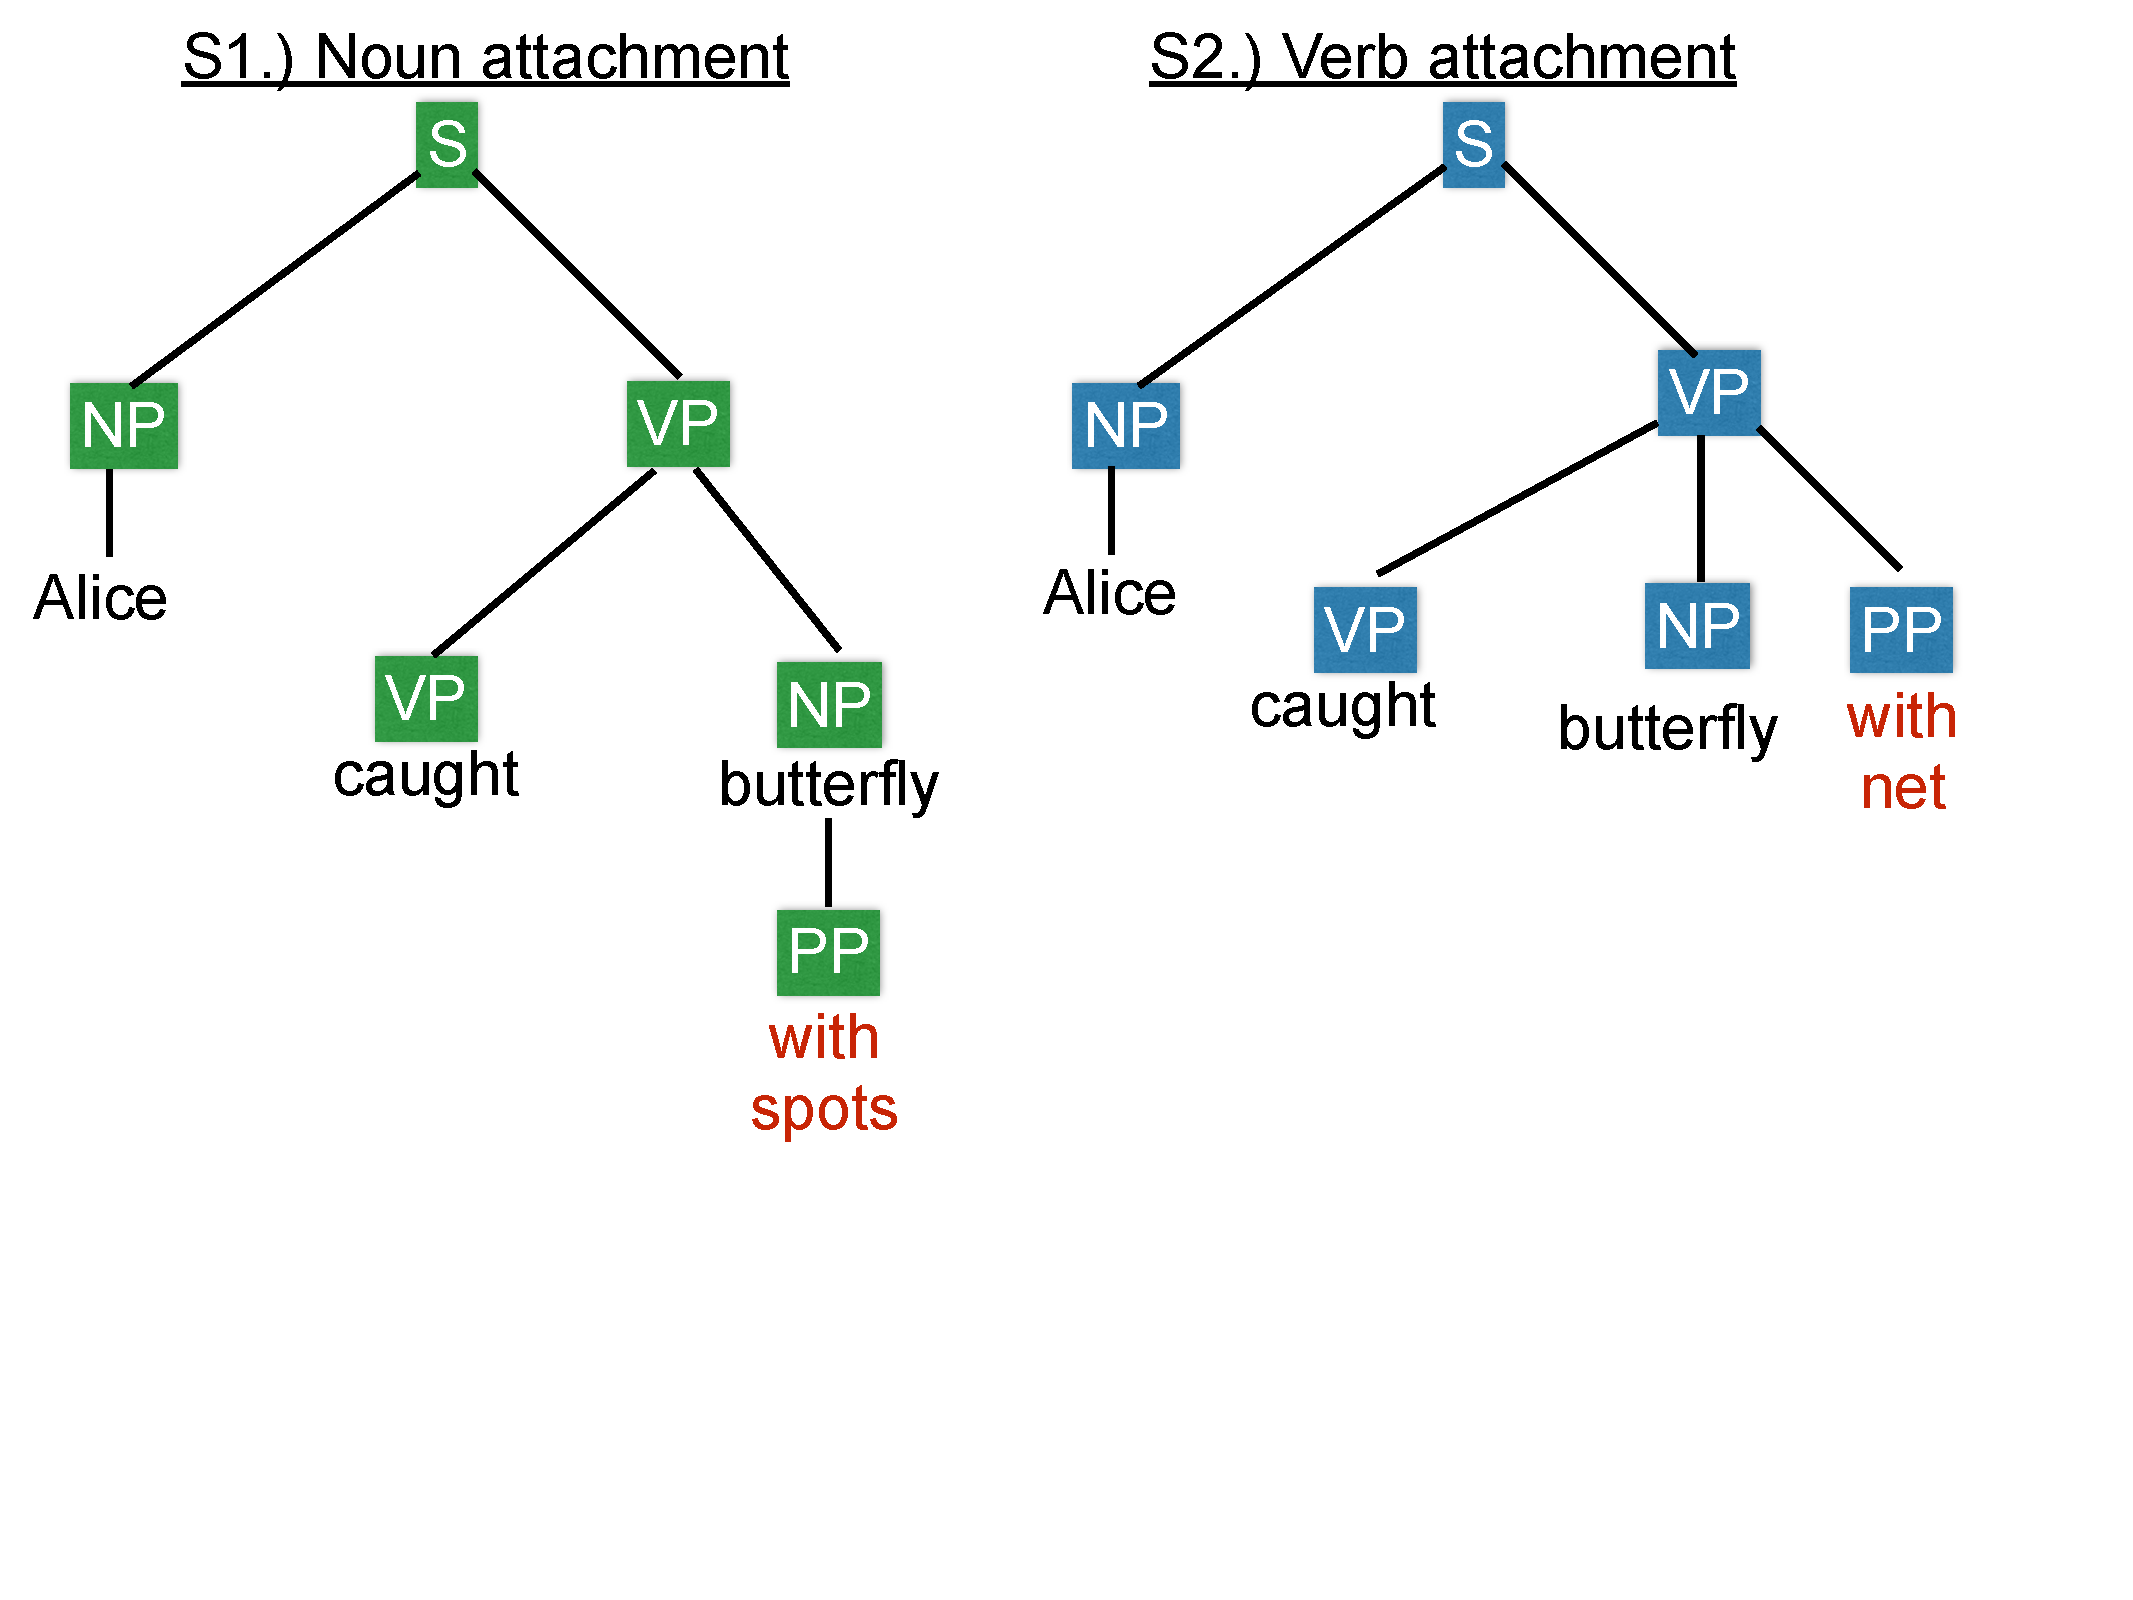
\includegraphics[width=1\columnwidth] {trees2.pdf}
\vspace*{-2.6cm}
\caption{Parse trees where the prepositional phrase (PP) attaches to the noun, and to the verb.}
%The only difference in the parse trees are the PP attachment sites, resulting in trees of different structures.}
%and hence the sentence structures are different. } 

\label{fig:deptrees}

\end{figure}



 As an example, consider the following sentences: \textit{ S1.) Alice caught the butterfly with the spots. S2.) Alice caught the butterfly with the net. }  S1 and S2 are syntactically different, this is evident from their corresponding parse trees in Figure \ref{fig:deptrees}. Specifically,  S1 and S2  differ in where their PPs attach. In  S1,  the butterfly has spots and therefore  the PP, ``with the spots'', attaches to the \textit{noun}. For relation extraction, we  obtain a \textit{binary} relation of the form:  
 $\langle$Alice$\rangle$  caught $\langle$butterfly with  spots$\rangle$.
However, in S2, the net is the instrument used for catching and therefore  the PP,  ``with the net", attaches to the \textit{verb}.  For relation extraction, we get a \textit{ternary} extraction of the form:
%\begin{itemize}
%\item[]
 $\langle$Alice$\rangle$  caught $\langle$butterfly$\rangle$ with $\langle$net$\rangle$.
%\item[] $\langle$The government$\rangle$  discovered $\langle$irregularities$\rangle$ in $\langle$June$\rangle$
%\end{itemize
 
The PP attachment problem is often defined as follows: given a PP occurring within a  sentence where there are multiple possible attachment sites for the PP, choose the most plausible attachment site. 
%Notice that in the examples we have given so far, there were only two possible attachment sites, the noun and the verb.
% as shown in Figure \ref{fig:deptrees} with a parse tree corresponding to each type.
 In the literature,  prior work going as far back as \cite{BrillR94,Ratnaparkhi1994,Collins95} has  focused on the  language pattern that causes most PP ambiguities, which is the  4-word sequence: $\{v, n1, p, n2\}$ (e.g., $\{${\em caught, butterfly, with, spots}$\}$). The task is  to   determine if  the prepositional phrase $(p,n2)$  attaches to  the verb $v$ or to the first noun $n1$.
Following common practice,  we focus on  PPs occurring as $\{v,n1,p,n2\}$ quadruples ---  we shall refer to these as  \textit{PP quads}. 

The approach we present here differs from prior work in two main ways. First, we make extensive use of semantic knowledge about nouns, verbs, prepositions, pairs of nouns, and  the discourse context in which a PP quad occurs. Table \ref{tab:knowledge}  summarizes the types of  knowledge we considered in our work. Second, in training our model, we rely on both labeled and unlabeled data, employing an expectation maximization (EM) algorithm \cite{Dempster77maximumlikelihood}. 


\begin{table}[h]
\centering
\small{
   \begin{tabular}{|p{1.8cm}|p{4.9cm}|}
     % \hline
   %&  {\bf Definition \& Example(s)}  \\
     \hline
    % \newline -receive(agent, patient, source) \\
     % \newline -isA(tea,beverage)\\
     Relations &  Noun-Noun binary relations  \newline \textit{ (Paris, located in, France)} \newline \textit{(net, caught, butterfly)}\\
     \hline
     Nouns &  Noun semantic categories \newline \textit{(butterfly, isA, animal)}  \\
     \hline
     Verbs & Verb roles \newline  \textit{caught(agent, patient, instrument)} \\
     \hline
     % \newline -(fork, used for, eating) \\
     Prepositions& Preposition  definitions \newline  
     \textit{ f(for)= used for, has purpose, ...}  
     \newline \textit{f(with)= has, contains, ...}  \\
     \hline
     Discourse &  Context \newline  $n0 \in \{n0, v, n1, p, n2\}$\\
     \hline
   \end{tabular}
   \caption{Types of background   
   knowledge used in this paper to determine PP attachment.}
     \label{tab:knowledge}
     }      
   \end{table}   
   

\begin{figure}[t]
%
\centering
%
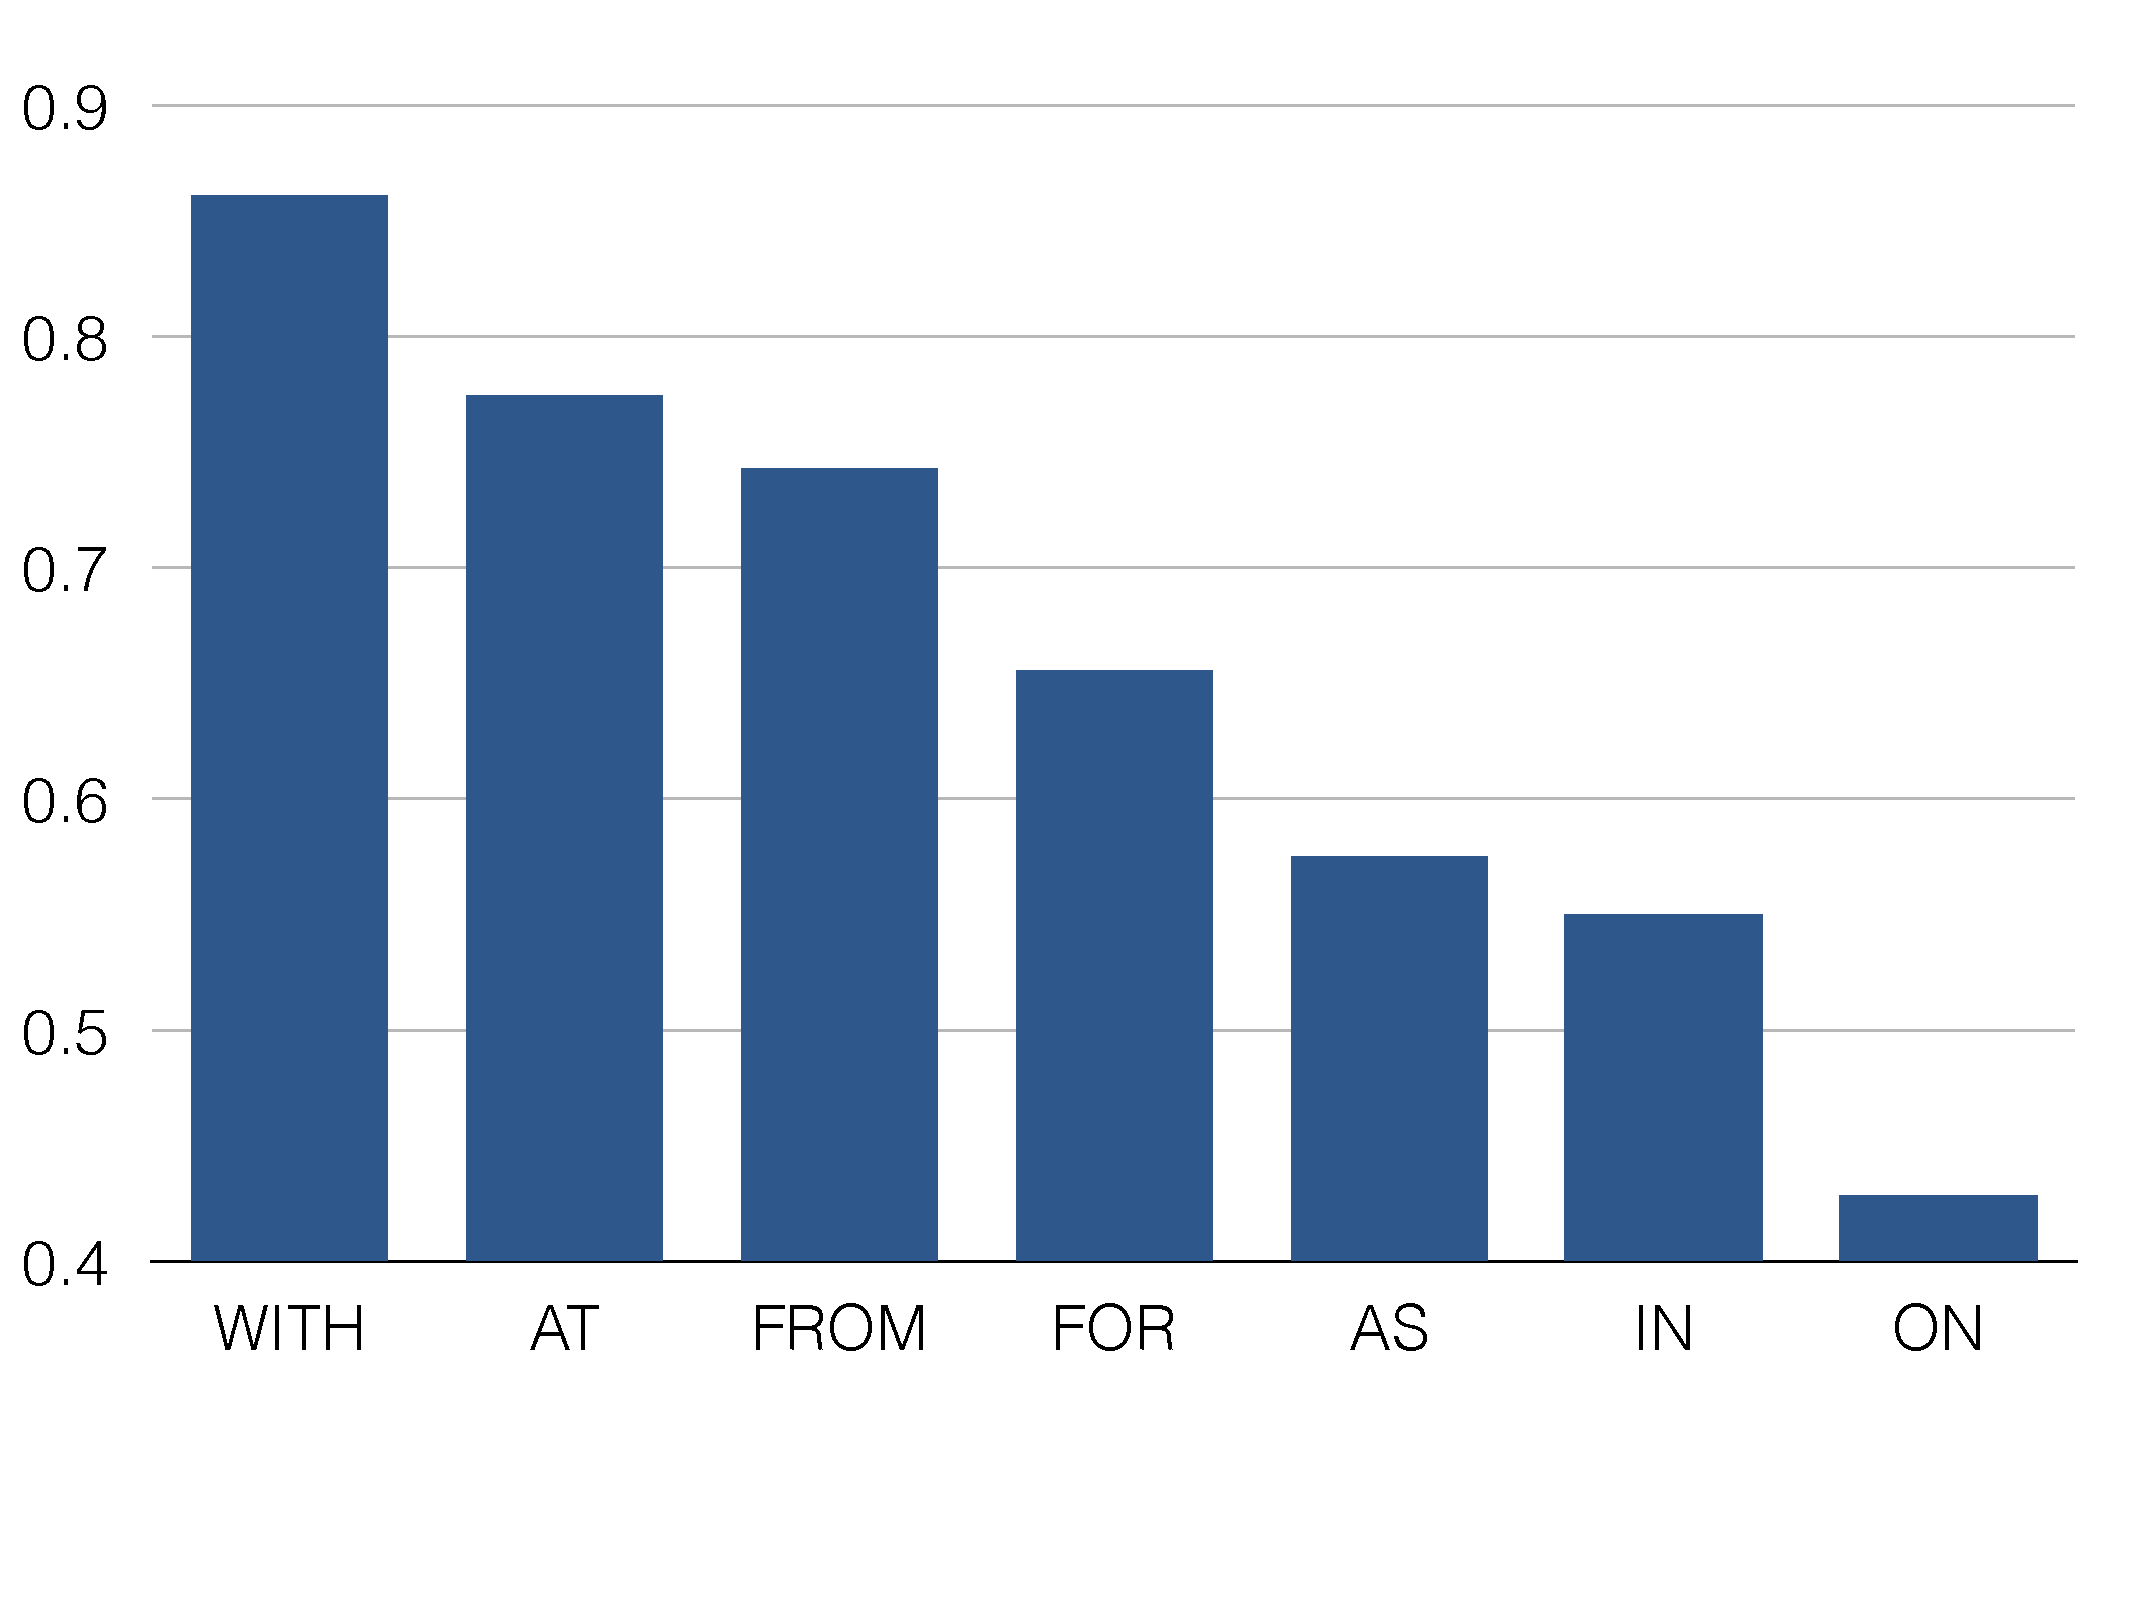
\includegraphics[width=0.80\columnwidth] {mainresults-0.pdf}
\vspace*{-0.8cm}
\caption{Dependency parser PP attachment accuracy for various frequent prepositions.}
% The only difference in the parse trees are the PP attachment sites, resulting in trees of different structures.}
% and hence the sentence structures are different. } 
%
\label{fig:parser}
%
\end{figure}  

                

\subsection{State  of  the Art}
    

\begin{figure}[t]
 %
 \centering
 %
 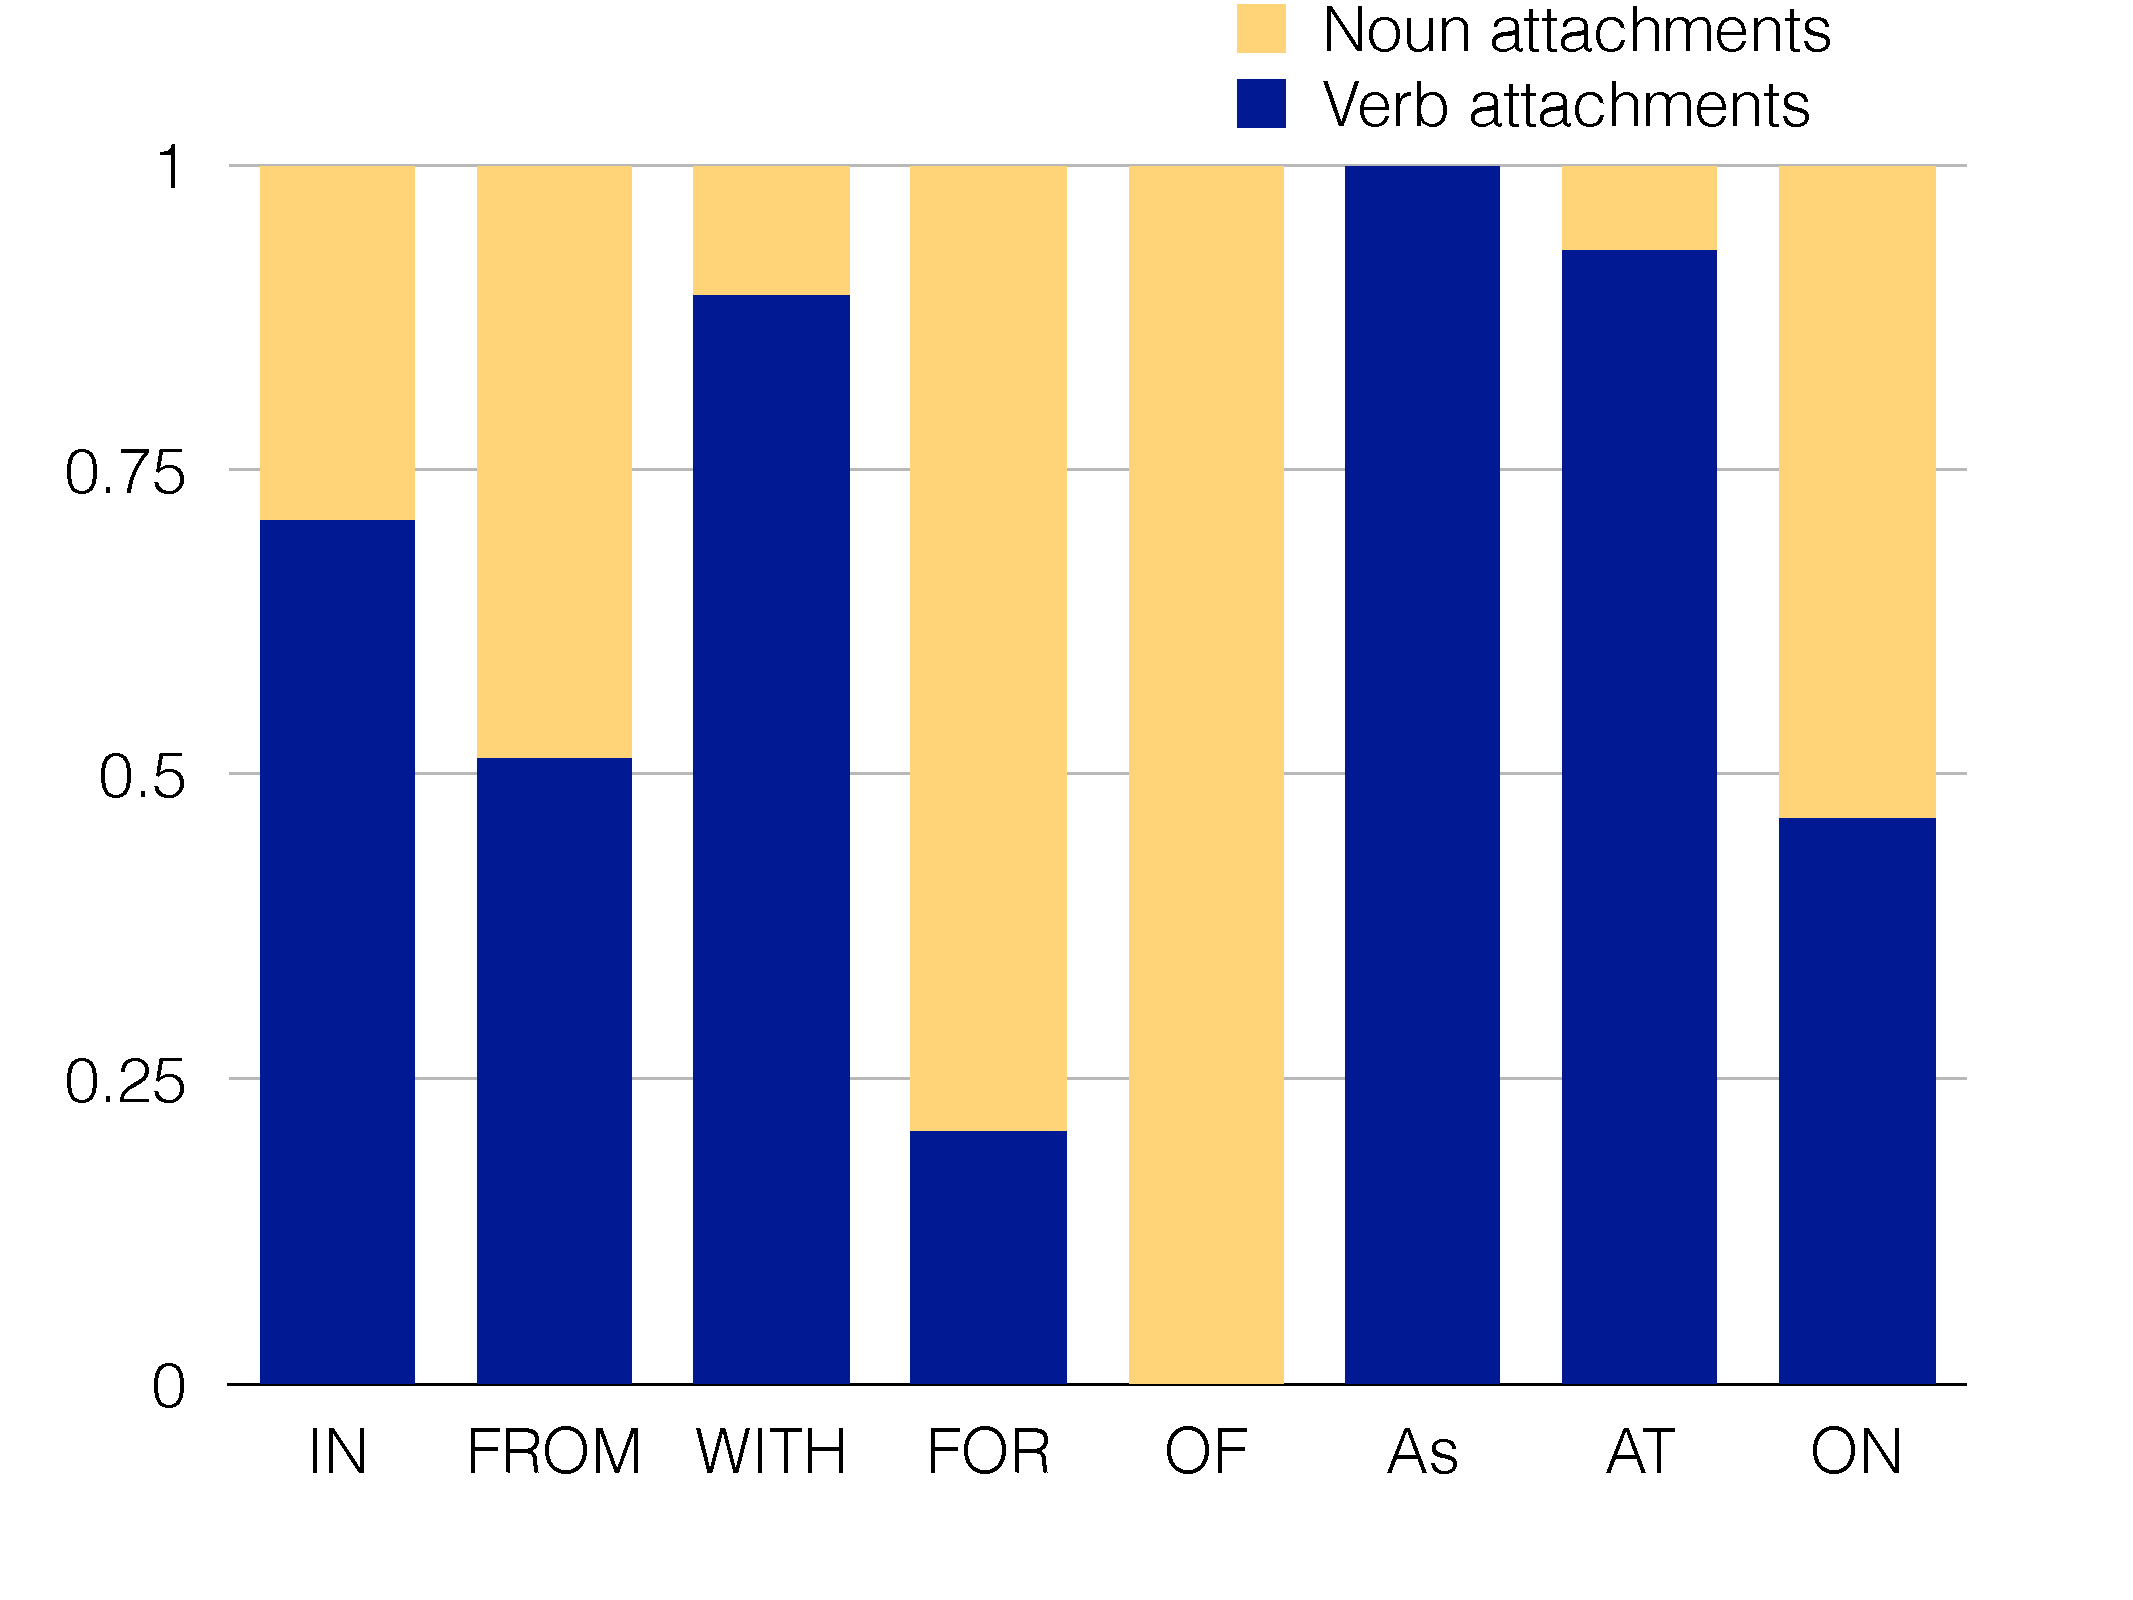
\includegraphics[width=0.85\columnwidth] {mainresults-5.pdf}
 \vspace*{-0.5cm}
 \caption{Noun vs. verb attachment proportions for frequent prepositions in the labeled NYTC dataset.}
 % The only difference in the parse trees are the PP attachment sites, resulting in trees of different structures.}
 % and hence the sentence structures are different. } 
 %
 \label{fig:distribution}
 %
 \end{figure}  

 To quantitatively assess existing tools, we analyzed performance of the widely used  Stanford parser\footnote {http://nlp.stanford.edu:8080/parser/} as of 2014,  and the established  baseline algorithm \cite{Collins95}, which has stood the test of time.
We first manually labeled PP quads from the NYTC dataset, then prepended the noun phrase appearing before the quad, effectively creating sentences made up of 5 lexical items 
$(n0\  v\  n1\  p\  n2)$.  We then applied the Stanford parser, obtaining the results summarized in Figure~\ref{fig:parser}.  The parser performs well on some prepositions, for example,  ``of", which tends to occur with noun attaching PPs as can be seen in Figure \ref{fig:distribution}.  However, for  prepositions  with an even distribution over verb and noun attachments, such as ``on", precision is as low as ~50\%. %indicating there is room for improvement.
The Collins baseline achieves 84\% accuracy on the benchmark Wall Street Journal PP dataset.  
 However, drawing a distinction in the precision of  different prepositions provides useful insights on its performance.  We re-implemented this baseline  and found that when we remove the trivial preposition,  ``of",  whose PPs are by default attached to the noun by this baseline, precision drops to 78\%. 
 This  analysis  suggests there is substantial room for improvement.
 % \highlight{For higher resolving prepositions.}


\subsection{Related Work}
\paragraph{Statistics-based Methods}
%common types of PP attachment methods in literature. 
Prominent  prior methods learn to perform PP attachment based on corpus co-occurrence statistics,  gathered either from  manually annotated training data \cite{Collins95,BrillR94} or from  automatically acquired  training data that may be noisy \cite{Ratnaparkhi98,PantelL00}.  These models collect statistics on how often a given quadruple, $\{v,n1,p,n2\}$, occurs in the training data as a verb attachment as opposed to a noun attachment.  The issue with this approach is sparsity, that is, many quadruples occuring in the test data might not have been seen in the training data.
Smoothing techniques are often employed to overcome sparsity.  For example, \cite{Collins95} proposed a back-off model that uses  subsets of the words in the quadruple, by also keeping  frequency counts of triples, pairs and single words. 
% when the test quadruple itself was not seen in the training data. 
Another approach to overcoming sparsity has been to use WordNet \cite{fellbaum98wordnet} classes, by replacing nouns with their WordNet classes \cite{Stetina97,ToutanovaMN04} to obtain less sparse corpus statistics.  Corpus-derived clusters of similar  nouns and verbs have also been used  \cite{PantelL00}.

Hindle and Rooth  proposed a lexical association approach based on how words are associated with each other \cite{HindleR93}. Lexical preference is used by  computing co-occurrence
frequencies (lexical associations) of verbs and nouns,  with prepositions. In this manner, they would discover that, for example,  the verb ``send" is highly associated with the preposition \textit{from},  indicating that in this case, the PP  is likely to be a verb attachment. 


\paragraph{Structure-based Methods}
These methods are based on  high-level  observations that are then generalized into heuristics for 
 PP attachment decisions. \cite{Kimball73}  proposed a right association method, whose premise is that a word tends to attach to another word immediately to its right.
\cite{Frazier78} introduced a minimal attachment method, which posits that  words attach to an existing non-terminal word using the fewest additional syntactic nodes. 
While simple, in practice these methods have been found to perform poorly \cite{WhittemoreFB90}.

\paragraph{Rule-based Methods}
%Different from frequency counting,
\cite{BrillR94}  proposed methods that
 learn  a set of transformation rules from a corpus. 
 %The  rules are then applied to a given PP attachment instance.
 %  and therefore, unlike the statistical methods, it is
%not necessary to store   tables  word dependencies or co-occurrence probabilities.
The rules can be too  specific to have broad applicability, resulting in low recall. 
To address low recall, knowledge about nouns, as found in  WordNet,   is used to replace certain
words in rules with  their WordNet classes. 
%This allows rules to match more  PP attachment instances


\paragraph{Parser Correction Methods}
The  quadruples formulation of the PP problem  can be seen as a simplified setting. This is because, with quadruples,  there is no need to deal with complex sentences but only well-defined quadruples of the form $\{v,n1,p,n2\}$. Thus in the quadruples setting, there are only two possible attachment sites for the PP, the $v$ and $n1$.  An alternative setting is to  work in the context of full sentences. In this setting the problem is cast as a dependency parser correction problem \cite{AttererS07,Agirre08,AnguianoC11}. That is, given a dependency parse of a sentence, with potentially incorrect PP attachments, rectify it such that the prepositional phrases attach to the correct sites. Unlike our approach, these methods do not take semantic knowledge into account.

\paragraph{Sense Disambiguation}
In addition to prior work on prepositional phrase attachment, a highly related problem is preposition sense disambiguation \cite{Hovy2011,SrikumarR13}.  Even a
syntactically correctly attached PP can  still  be semantically ambiguous with respect to questions of machine reading such as \textit{where, when,} and \textit{why}. 
Therefore, when extracting information from prepositions, the problem of preposition sense disambiguation (semantics) has to be addressed in addition to prepositional phrase attachment disambiguation (syntax). In this paper, our focus is on the latter. 

\begin{table*}[th]
%
\centering
%
\begin{tabular}{ |l| l|l|l| }
\hline
{\bf Feature Type} & {\bf \#} &  {\bf Feature}  & {\bf Example}\\
\hline

Noun-Noun Binary Relations &  & \textbf{Source: SVOs} & \\ 
   & F1. &  $svo(n2,v,n1)$  &  For q1; $(net,caught,butterfly)$\\ 
 % & $svo(t2,v,t1)$  &  For q1; $svo(< device>,caught, <animal>)$\\ 
& F2. &  $\forall i : \exists sv_{i}o; $  $svo(n1,v_i,n2)$ & For q2; $(butterfly,has,spots)$ \\ 
%& & & For q2; $(butterfly,can $ $have,spots)$\\ 
& & & For q2; $(butterfly, can $ $see,spots)$\\ 

   Noun  Semantic Categories  &  &  {\bf Source: $\mathcal{T}$ }  & \\
                & F3. &  $\forall t_i \in \mathcal{T};$ $isA(n1,t_i)$ & For q1 $isA(butterlfy,animal)$\\ 
                   & F4. &  $\forall t_i \in \mathcal{T};$  $isA(n2,t_i)$ & For q2 $isA(net,device)$\\ 
                                                                                                          
  Verb  Role Fillers & & \textbf{Source: VerbNet} & \\ 
  & F5. &   $hasRole(n2, r_{i})$ &  For q1; $(net, instrument)$ \\
%   &  &  &   For q3; $(child, beneficiary)$ \\   

Preposition Relational  &  &  \textbf{Source: $\mathcal{M}$} & \\ 
  Definitions & F6. & $def(prep,v_i)$ $\forall i :$ &  
\\ 
         &  & $\exists sv_{i}o; v_i \in  \mathcal{M}$ $ \wedge$  &  
       \\ 
          &  &  $svo(n1,v_i,n2)$  &  For q2;
                    $def(with,has)$ \\ 
 % &  &  $svo(n1,v_i,n2)$  & For q2; $(butterfly,can $ $have,spots)$\\  
 
 Discourse Features &  & \textbf{Source: Sentence(s), $\mathcal{T}$} & \\ 
             & F7. &  $\forall t_i \in \mathcal{T}; isA(n0,t_i)$ &  $n0 \in \{n0, v, n1, p, n2\}$ \\
             %$isA(n0,t_i)$ & For  $n0 \in \{n0, v, n1, p, n2\}$ \\

Lexical  Features& &  {\bf Source: PP quads} & For q1;\\ 
& F8.  & $(v, n1, p, n2)$ & $(caught,butterfly,with,net)$ \\
& F9. & $(v, n1, p)$ & $(caught,butterfly,with)$ \\
& F10. & $(v, p, n2)$ & $(caught,with,net)$ \\ 
& F11. & $(n1, p, n2)$ &$(butterfly,with,net)$ \\ 
& F12.  & $(v,p) $ & $(caught,with)$\\ 
& F13.  & $(n1,p) $ & $(butterfly,with)$\\ 
& F14. & $(p,n2) $ & $(with,net)$ \\ 
   &F15.  &$(p) $ & $(with)$\\  
\hline
\end{tabular}
\caption{Types of  features considered in our experiments. All features have values of 1 or 0.  The PP quads used as running examples are:  $q1=\{caught, butterfly, with, net\}: V$, $q2=\{caught, butterfly, with, spots\}: N$.}
\label{tab:featurevectors}
\end{table*}
   
 

\subsection{Methodology} 
%\highlight{Do not refer to features but rather to feature types.}
%Attributes, Ownership/Possession
%[NP’s NP]: Mary’s laptop or car’s wheel  but also Mary’s brother or  France’s political elite, government 's explanation,  Netanyahu 's frosty visit 
%[NP of NP]:  eyes of the baby, economy of Asia,  but also fact of life, a lot of chances 
%[NP has/have NP]:  Bob has brown eyes, Bob has a cat, cats have fur, cake has nuts, 
%[NP is made of NP]: foil made of aluminum 
%[NP contains/consists of NP]:  wine contains alcohol, water consists of hydrogen



Our approach consists of first generating features from background knowledge and then training a model to learn with these features.
%extracted from both labeled and unlabeled data. 
 The types of features considered in our experiments are  summarized  in Table~\ref{tab:featurevectors}.  The choice of features was motivated by our empirically driven characterization of the problem as follows:
\begin{table}[h]
\centering
\begin{tabular}{p{7cm}}
\textit{(Verb attach) $\longrightarrow$ v $\langle$has-slot-filler$\rangle$ n2} \\
\hline
\textit{(Noun attach a.) $\longrightarrow$ n1 $\langle$described-by$\rangle$ n2}\\
\textit{(Noun attach b.) $\longrightarrow$ n2 $\langle$described-by$\rangle$ n1}\\
\end{tabular}
\label{tbl:example}
\end{table}

That is, we found that for verb-attaching PPs, $n2$  is usually a role filler for the verb, e.g., the net fills the role of an instrument for the verb $catch$. On the other hand,  for noun-attaching PPs,  one noun describes or elaborates on the other. In particular, we found  two kinds of noun attachments. For the first kind of noun attachment,  the second noun $n2$ describes  the first noun $n1$, for example $n2$ might be  an attribute or property of $n1$, as in   the spots($n2$) are an attribute of the butterfly ($n1$).  And for the second kind of noun attachment, the first noun $n1$ describes the second noun $n2$, as  in the PP quad $\{${\em expect, decline, in, rates}$\}$,  where the PP ``in rates'', attaches to the $noun$. The decline:$n1$ that is expected:$v$ is in the rates:$n2$. We sampled $50$ PP quads from the WSJ dataset and found that every labeling could be explained using our characterization.  
 We make this labeling available with the rest of the datasets.



We next describe in more detail how each type of feature is derived from the  background knowledge  in Table~\ref{tab:knowledge}.

We generate boolean-valued features for all the feature types we describe in this section.

\subsubsection{Noun-Noun Binary Relations}
%This type of knowledge refers to binary relations between pairs of nouns. 
The noun-noun  binary relation features, F1-2 in Table \ref{tab:featurevectors}, are boolean features   $svo(n1,v_i,n2)$ (where $v_i$ is any verb) and $svo(n2,v,n1)$ (where $v$ is the verb in the PP quad, and the roles of $n2$ and $n1$ are reversed). These features describe diverse semantic relations between pairs of nouns (e.g.,   \textit{butterfly-has-spots},   \textit{clapton-played-guitar}).  To obtain this type of knowledge, we dependency parsed all sentences in the 500 million English web pages of the ClueWeb09 corpus, then extracted subject-verb-object (SVO) triples from these parses, along with the frequency of each SVO triple in the corpus.  The value of any given feature $svo(n1,v_i,n2)$ is defined to be 1 if that SVO triple was found at least $3$ times in these SVO triples, and 0 otherwise.


To see why these relations are relevant, let us suppose that  we have  the knowledge that \textit{butterfly-has-spots}, $svo(n1,v_i,n2)$. From this, we can  infer that the PP in $\{caught,butterfly, with, spots\}$ is likely to attach to the noun.   Similarly,  suppose we  know that \textit{net-caught-butterfly}, $svo(n2,v,n1)$. The fact   that a net can be used to catch a butterfly can be used to predict that  the  PP in\\ $\{caught,butterfly, with, net\}$ is likely to attach to the verb.   

\subsubsection{Noun Semantic Categories} 

Noun semantic type features, F3-4, are boolean features   $isA(n1,t_i)$ and $isA(n2,t_i)$ where $t_i$ is a noun category in a noun categorization  scheme   $\mathcal{T}$ such as WordNet classes. 
Knowledge about semantic types of nouns, for example  that a butterfly is an animal, enables extrapolating predictions to other PP quads that contain nouns of the same type. % For example,  $\{caught,<$$animal$$>, with, spots\}$. 
We ran experiments with several noun categorizations including WordNet classes,  knowledge base ontological types,  and an unsupervised noun categorization produced by clustering  nouns based on the verbs and adjectives with which they co-occur  (distributional similarity).  

\subsubsection{Verb Role Fillers} 
The verb role feature, F5, is a boolean feature $hasRole(n2, r_{i})$ where $r_i$ is a role that  $n2$ can fulfill for the verb  $v$ in the PP quad, according to background knowledge. Notice that  if  $n2$ fills a role for the verb, then the PP is a verb attachment.  Consider the quad $\{caught,butterfly, with, net\}$, if we know that  a net can play the role of an \textit{instrument} for the verb \textit{catch}, this suggests a likely verb attachment.  We obtained background knowledge of verbs and their possible roles  from the VerbNet lexical resource ~\cite{KipperKRP08}. 
From VerbNet we obtained $2,573$ labeled  sentences containing PP quads (verbs in the same VerbNet group are considered synonymous), and the  labeled semantic roles  filled by the second noun $n2$ in the PP quad.  We use these example sentences  to label similar  PP quads, where similarity of PP quads is defined by  verbs from the same VerbNet group. 

%See feature 5 in Table~\ref{tab:featurevectors}.

\subsubsection{Preposition  Definitions}
The preposition  definition feature, $F6$, is a boolean feature $def(prep,v_i)=1$ $if$ $\exists v_i \in  \mathcal{M}$ $ \wedge$  $svo(n1,v_i,n2)=1$, where $ \mathcal{M}$ is a definition mapping of prepositions to verb phrases.   This mapping defines prepositions, using verbs in our ClueWeb09 derived SVO corpus, in order to capture their senses using verbs; it contains definitions such as \textit{def(with, *) = contains, accompanied by, ... }.   If  ``with" is  used in the  sense of ``contains" , then the PP  is a likely noun attachment, as in $n1$ contains $n2$ in the quad $ate, cookies, with, cranberries$. However, if  ``with" is  used in the sense of  ``accompanied by", then the PP is a likely verb attachment, as in the quad $visted, Paris, with, Sue$.

% when used in conjunction with  binary relation features.
To obtain the mapping, we took the labeled PP quads (WSJ, \cite{Ratnaparkhi1994}) and computed a ranked list of verbs from SVOs, that appear frequently between  pairs of nouns  for a given preposition.
 %, for a given attachment site verb(v) or noun(n). 
 % We obtained a large collection of such mappings.
 Other   sample mappings are:  \textit{def(for,*)= used for},   \textit{def(in,*)= located in}. Notice that this feature $F6$ is a selective, more targeted version of $F2$.
 %\textit{f(from,n)= comes from, born in, ...}.




\subsubsection{Discourse and Lexical Features}
The  discourse feature, $F7$,  is  a boolean feature  $isA(n0,t_i)$, for each noun category $t_i$ found in a noun category ontology  $\mathcal{T}$  such as WordNet semantic types. 
The context of the PP quad can contain relevant information  for  attachment decisions. We  take into account the noun preceding  a PP quad, in particular, its semantic type. This in effect makes the PP quad into a  PP 5-tuple:  $\{n0, v, n1, p, n2\}$, where the $n0$  provides additional context.
% See feature $7$ in Table~\ref{tab:featurevectors}.

%\subsection{}
%\subsubsection{ Features}
Finally, we  use  lexical features in the form of PP quads, features F8-15.  To overcome sparsity of  occurrences of PP quads, we also use counts of shorter sub-sequences, including  triples, pairs and singles. We only use sub-sequences that contain the preposition, as the preposition has been found to be highly crucial in PP attachment decisions \cite{Collins95}.
% See features $8-15$ in Table~\ref{tab:featurevectors}.
   
\subsection{Disambiguation Algorithm}
We use the described features to train a  model for  making PP attachment decisions.
Our goal is to compute $\mathbb{P}(y|x)$,   the probability that the PP $ (p,n2)$ in the tuple $\{v,n1,p,n2\}$ attaches to the  \textit{verb (v)} , $y=1$ or  to the $noun (n1)$, $y=0$, given a feature vector $x$ describing that tuple.
As input to training the model, we are given a collection of PP quads, $D$ where  $d_i \in \mathcal{D}: d_i=\{v,n1,p,n2\} $. A small subset,
$D^l \subset \mathcal{D}$   is labeled data, thus for each $d_i \in D^l$ we know the corresponding $y_i$. The  rest of the quads, $D^u$,  are unlabeled, hence their corresponding $y_i$s are unknown.
%In short, we have a  disjoint partitioning such that $\mathcal{D} = D^l \cup D^u $, where $|D| =N$  or equivalently,   $|D^l \cup D^u| = N$, and $|D^l| << |D^u|$.
From each PP quad $d_i$, we extract a feature vector $x_i$ according to the feature generation process  discussed earlier.. 
%Thus we have  feature vectors $\mathcal{X} =\{ x_1, .., x_N\}$.

\subsubsection{Model}
To  model $\mathbb{P}(y|x)$, there a various possibilities. One could use a generative model (e.g., Naive Bayes) or a discriminative model ( e.g., logistic regression). In our experiments we used both kinds of models, but found the discriminative model performed better. Therefore, we present details only for our discriminative model.  We use the  logistic function: 
%$\mathbb{P}(y|x, \vec \theta)  =  \frac{e^{\vec \theta x}}{1+ e^{\vec \theta x}}$,
 \begin{equation*}
 \mathbb{P}(y|x, \vec \theta)  =  \frac{e^{\vec \theta x}}{1+ e^{\vec \theta x}}
\end{equation*}
 where $\vec \theta$  is a vector of model parameters. To estimate these parameters,  we could use the labeled data as training data and  use standard   gradient descent  to minimize the logistic regression cost function. However, we also leverage the unlabeled data.  

 
 \subsubsection{Parameter Estimation}
 To estimate model parameters based on both labeled and unlabeled data, we use an Expectation Maximization (EM) algorithm. 
% The EM algorithm enables parameter estimation in models with incomplete data. 
 %In our case, the data is incomplete because the $D^u$ labels are unknown. 
 EM estimates model parameters that maximize the expected log likelihood of the full (observed and unobserved) data.  

Since we are using a discriminative model, our likelihood function is  a  conditional likelihood function:
  \begin{align}\label{eqlikelihood}
  \mathcal{L}(\theta)  &=\sum_{i=1}^{N} \mbox{ln }  \mathbb{P}(y_i|x_i)  \nonumber \\
     &= \sum_{i=1}^{N}  y_i \theta^{T}x_i - \mbox{ln } (1+ exp ( \theta^{T}x_i)) 
   \end{align}
where $i$ indexes over the $N$ training examples.
  
  

The  EM algorithm produces parameter estimates that correspond to a local maximum in the expected log likelihood of the data under the posterior distribution of the labels, given by: \\   $\arg\max\limits_{\theta}  E_{p(y|x,\theta)} [ \mbox{ln } \mathbb{P}(y|x,\theta)]$.  In the E-step, we use the current parameters $\theta^{t-1}$ to compute the posterior distribution over the $y$ labels, give by $\mathbb{P}(y|x, \theta^{t-1})$.   We then use this posterior distribution to find the expectation of the log of the complete-data conditional likelihood, this expectation is given by  $\mathcal{Q}({\bf\theta, \theta^{t-1})}$, defined as:

  \begin{align}
\mathcal{Q}(\theta,  \theta^{t-1})  &=\sum_{i=1}^{N} E_{\theta^{t-1}} [ \mbox{ln } \mathbb{P}(y|x,\theta)]  
    \end{align}

In the M-step, a new estimate $\theta^t$ is then produced, by maximizing this $Q$ function with respect to $\theta$:
\begin{equation} \label{empameterupdate}
{\bf \theta^{t}} =\arg\max\limits_{\theta}\mathcal{Q}({\bf\theta, \theta^{t-1})}
\end{equation}

EM iteratively computes  parameters $\theta^0, \theta^1, ...\theta^{t}$,  using the above update rule at each iteration $t$, halting when there is no further improvement in the value of the $Q$ function.  Our algorithm is summarized in Algorithm 1.  The M-step solution for $\theta^t$ is obtained using gradient ascent to maximize the $Q$ function.  

 \begin{algorithm}
 \caption{The EM algorithm  for PP attachment}
 \label{algorithm}
 \begin{algorithmic}
 \STATE \textbf{Input:}  $\mathcal{X}, \mathcal{D} = D^{l} \cup D^{u}$\\
 %\STATE \textbf{Input:} Prior Knowledge  $\mathcal{K}$ \\
 \STATE \textbf{Output:} $\theta^{T}$
 %\STATE  $\mathcal{X} =getFeatureVectors(\mathcal{D})$
 %\STATE  $\mathcal{X} =\{ x_1, .., x_N\}$
 \FOR{t = 1 . . . T}
   \STATE \textbf{E-Step:}
   \STATE Compute $p(y|x_i, \theta^{t-1})$\\
   \STATE $x_i: d_i\in D^u$; $p(y|x_i, \vec \theta)  =  \frac{e^{\vec \theta x}}{1+ e^{\vec \theta x}}$  \\
   \STATE $x_i: d_i \in D^{l}$; $p(y|x_i)= 1$ if  $y=y_i,$ else $0$ \\
   \STATE \textbf{M-Step:} 
   \STATE Compute new parameters, $\theta^{t}$\\
   \STATE ${\bf \theta^{t}}$ $=\arg\max\limits_{\theta}\mathcal{Q}({\bf\theta, \theta^{t-1})}$
   \vspace{-0.4cm}
   \begin{multline*}
    \mathcal{Q}(\theta,  \theta^{t-1})  =\sum_{i=1}^{N}\sum_{y\in\{0,1\}}   p(y|x_i,\theta^{t-1}) \times\\( y\theta^{T}x_i - \mbox {ln}  (1+ exp ( \theta^{T}x_i)) ) 
   \end{multline*}
    		
     \IF{convergence($\mathcal{L}(\theta),  \mathcal{L}(\theta^{t-1}))$}
     	\STATE \textbf{break}\\
     \ENDIF
 \ENDFOR
 \RETURN $\theta^{T}$
 \end{algorithmic}
 \end{algorithm} 
 
 



\subsection{Experimental Evaluation}
We evaluated our method on several datasets containing PP quads of the form $\{v,n1,p,n2\}$.   The task is to predict if the  PP ($p,n2$) attaches to the verb $v$ or to the first noun $n1$. 


\subsubsection{Experimental Setup}\label{experimentalsetup}

\begin{table}[t]
%
\centering
%
\begin{tabular}{|l|l|l|}
\hline
{\bf DataSet} &  {\bf  \# Training quads} & {\bf \# Test quads} \\
\hline
\multicolumn{3}{|c|}{Labeled data} \\
    \hline
WSJ &  20,801 & 3,097 \\
NYTC & 0 & 293  \\
 WKP & 0 & 381  \\
      \hline
 \multicolumn{3}{|c|}{Unlabeled data} \\
      \hline
        %WSJ & - & - \\
         %NYTC & - & - \\
          WKP  & 100,000 & 4,473,072 \\
         
\hline
\end{tabular}
\caption{Training and test datasets used in our experiments. }
%\tom{What does "-" mean in this table?  If zero, let's use "0"}}
\label{tab:datasets}
\end{table}
     
    
     
\paragraph{Datasets}
Table~\ref{tab:datasets} shows the datasets used in our experiments. 
As labeled training data, we used the Wall Street Journal  (WSJ) dataset. For the unlabeled  training data, we extracted  PP quads from Wikipedia (WKP) and randomly selected $100,000$ which we found  to be a sufficient amount of unlabeled data.
The largest labeled test dataset is  WSJ
but it is also made up of a large fraction, of  ``of" PP quads, 30\% , which trivially attach to the noun, as already seen  in Figure \ref{fig:distribution}.
%and in general it is more comprehensive in the kind of prepositions it contains.
 The New York Times (NYTC) and Wikipedia (WKP) datasets are  smaller but contain fewer proportions  of ``of" PP quads, 15\%,  and 14\%, respectively. 
  %with a focus on  frequently used prepositions.
  Additionally, we applied our  model to over 4 million unlabeled 5-tuples from Wikipedia. We make this data available for download,  along with our manually labeled NYTC and WKP datasets.
For the WKP \& NYTC corpora,  each quad has a  preceding noun, $n0$, as context, resulting in PP 5-tuples of the form:  $\{n0,v,n1,p,n2\}$. The WSJ dataset was only available to us in the form of  PP quads with no other sentence information.

\begin{table}[t]
\centering
\begin{tabular}{|l|l|l|l|l|}
\hline
& PPAD& PPAD- &Coll-& Stan-\\
& & NB &ins& ford\\
\hline
WKP &  \bf{0.793} &	0.740&	0.727&	0.701\\
\hline
WKP  & \bf{0.759} &	0.698&	0.683&	0.652 \\
\textbackslash of  & & & & \\
\hline
NYTC & \bf{0.843}	& 0.792	&0.809	&0.679\\
\hline
NYTC& \bf{0.815}	& 0.754&	0.774&	0.621\\
\textbackslash of  & & & & \\
\hline
WSJ & \bf{0.843}&	0.816&	0.841& N\textbackslash A \\
\hline
WSJ & \bf{0.779}	& 0.741&	0.778&N\textbackslash A  \\
\textbackslash of  & & & & \\
\hline
\end{tabular}
 \caption{PPAD  vs. baselines.}
   \label{fig:resultmain}
\end{table}
    

\begin{figure}[t]
%
\centering
%
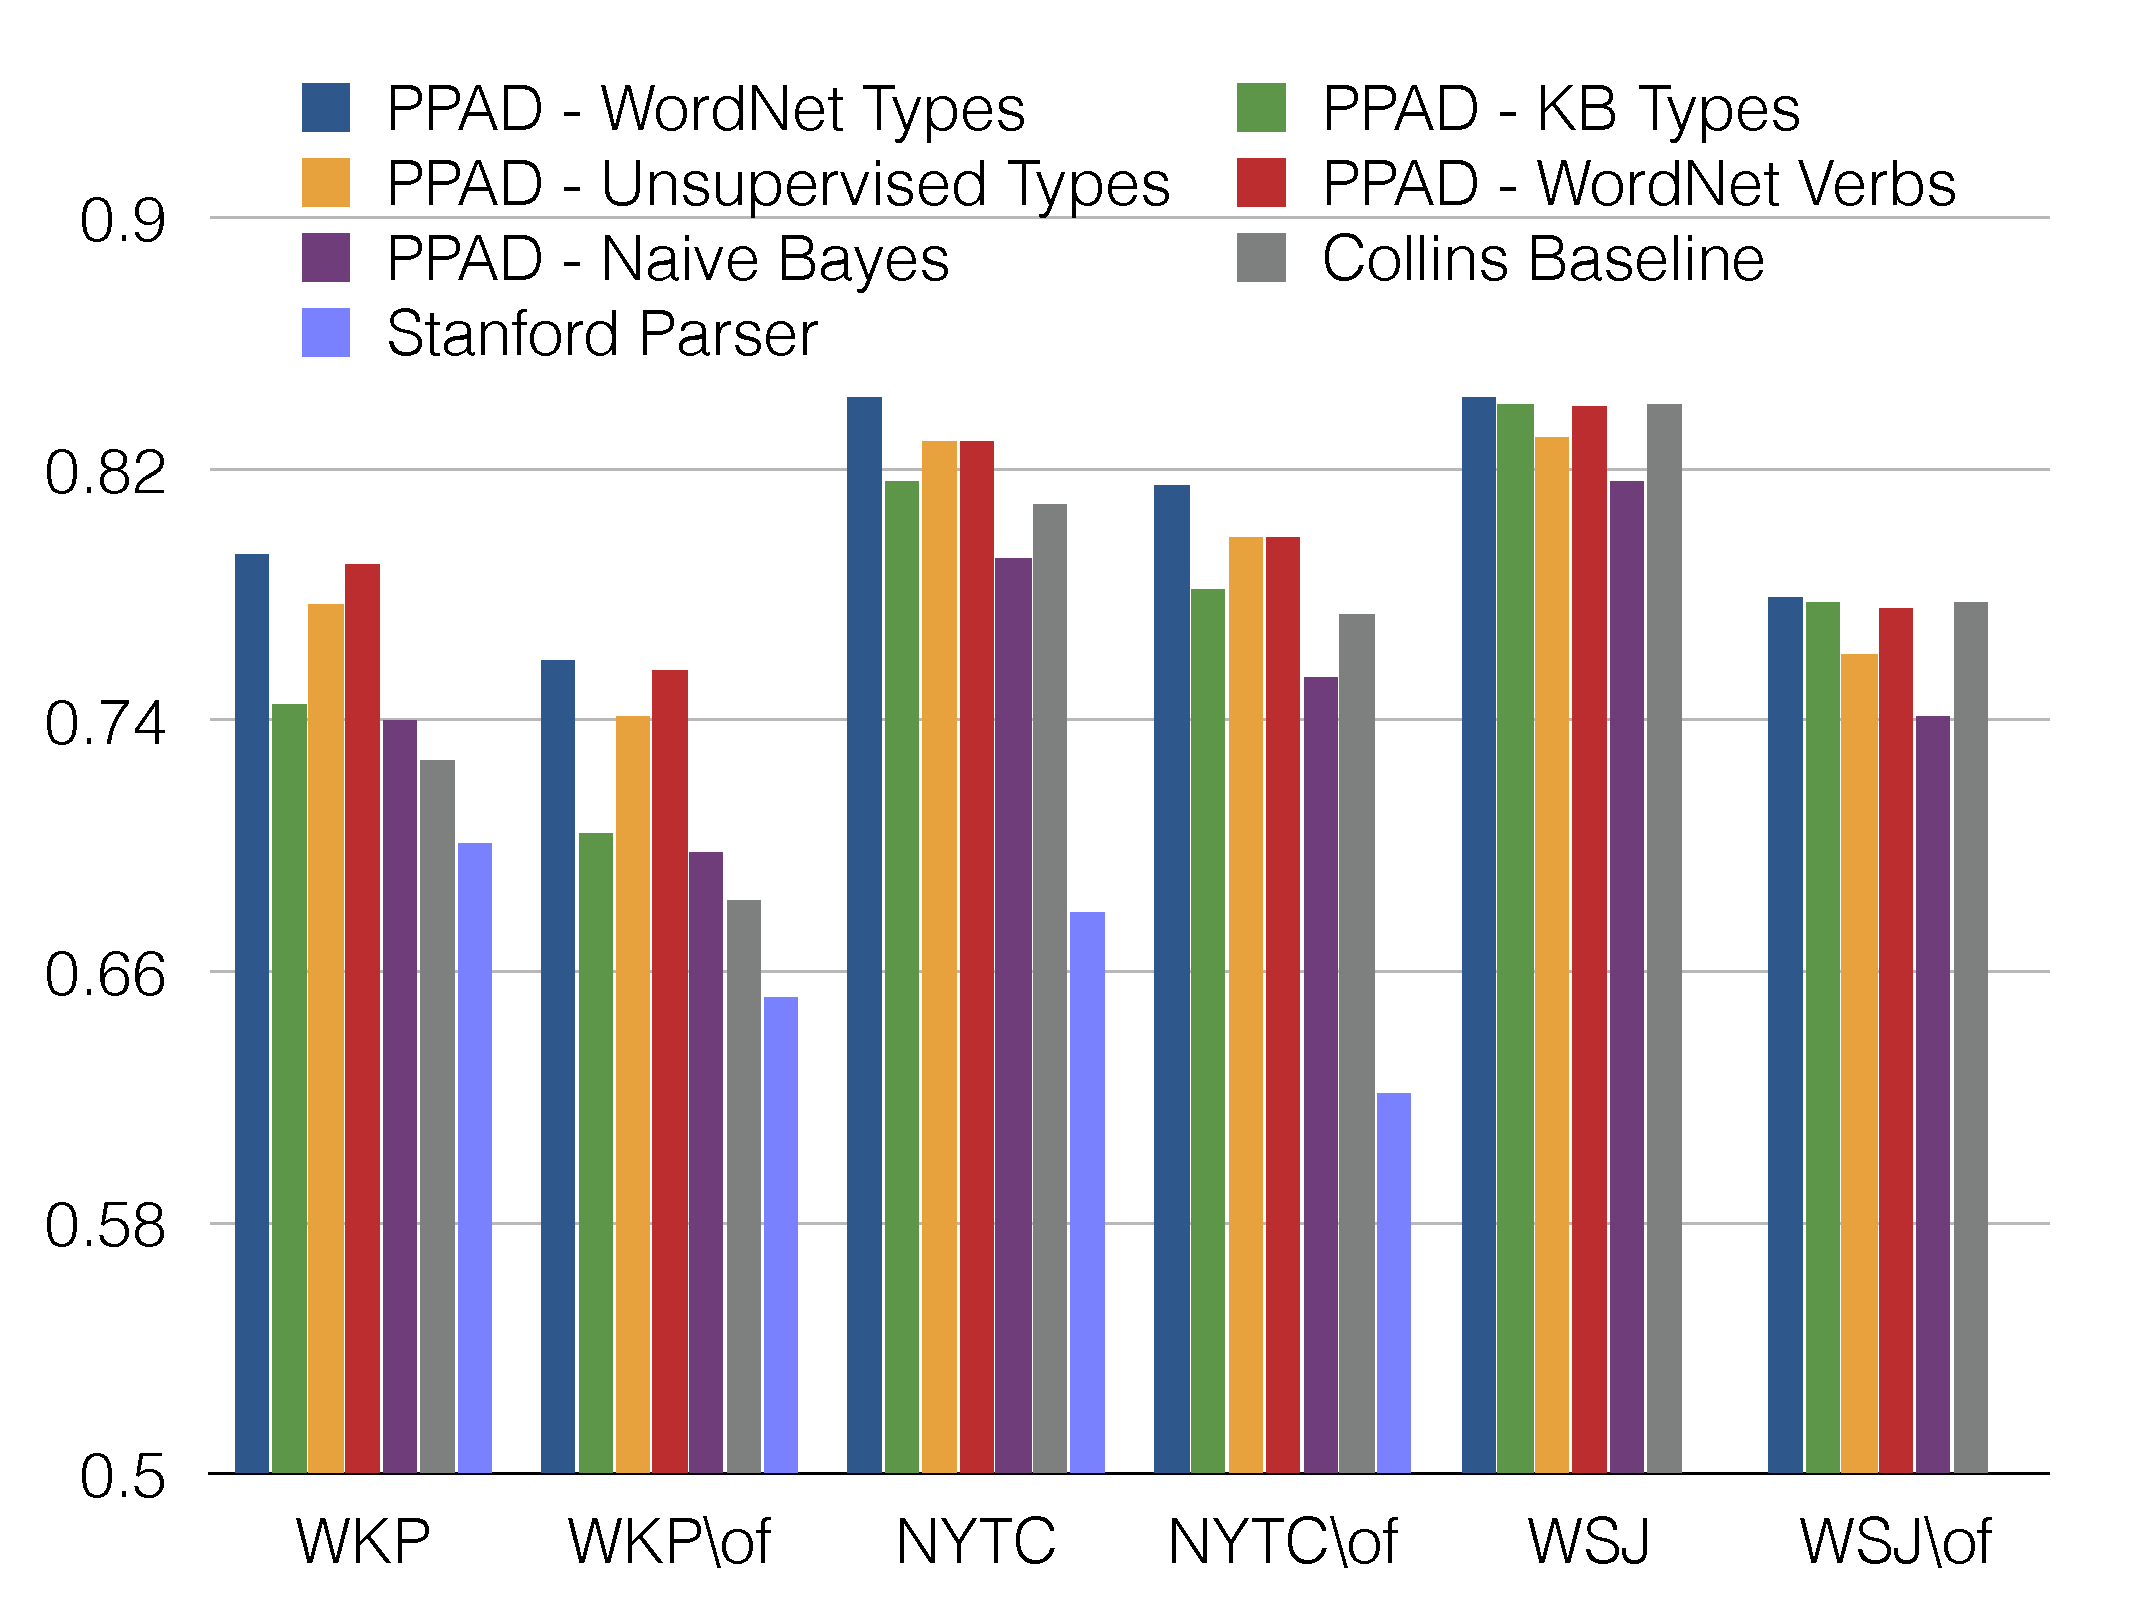
\includegraphics[width=1\columnwidth] {mainresults-2.pdf}
%
\vspace*{-1cm}
\caption{PPAD variations vs. baselines.}
%
\label{fig:resultmain2}
%
\end{figure}
    
   
    
 \paragraph{Methods Under Comparison} 
\textit{1) PPAD}  (Prepositional Phrase Attachment Disambiguator) is  our proposed method. It uses diverse types of semantic knowledge, a mixture of labeled and unlabeled data for training data, a logistic regression classifier, and expectation maximization (EM) for parameter estimation \textit{2) Collins} is the established baseline among PP attachment algorithms \cite{Collins95}.  \textit{3) Stanford Parser} is a state-of-the-art dependency parser, the 2014 online version. \textit{4) PPAD Naive Bayes(NB)}  is the same as PPAD but  uses a generative model,  as opposed to the discriminative model used in  PPAD.


 \subsubsection{PPAD vs. Baselines}
Comparison results of our method to the three baselines are shown in Table \ref{fig:resultmain}. For each dataset, we also show  results when the ``of" quads are removed, shown as ``WKP\textbackslash of'', ``NYTC\textbackslash of'', and ``WSJ\textbackslash of''.
 Our method yields  improvements over the baselines. Improvements are  especially significant on the datasets for which no labeled data was available  (NYTC and WKP). On  WKP, our method is 7\% and 9\% ahead of the Collins baseline and the Stanford parser, respectively.  On  NYTC, our method is 4\% and 6\% ahead of the Collins baseline and the Stanford parser, respectively. On WSJ, which is the source of the labeled data, our method  is not significantly  better than the Collins baseline. We could not evaluate the Stanford parser on the  WSJ dataset.  The parser requires well-formed sentences which we could not generate from the WSJ dataset as it was only available to us in the form of  PP quads with no other sentence information.  For the same reason,  we could not generate discourse features,$F7$, for the  WSJ PP quads.  For the  NYTC and WKP datasets, we generated well-formed short  sentences containing only the PP quad and the noun preceding it.  

 
 \subsubsection{Feature Analysis}
We found that features $F2$ and $F6$ did not improve performance, therefore we  excluded them from the final model, PPAD. This means that binary noun-noun relations were not useful when used permissively, feature $F2$, but when used selectively, feature $F1$, we found them to be useful. Our attempt at mapping prepositions to  verb definitions produced some noisy mappings, resulting in feature $F6$  producing mixed results.
To analyze the impact of the unlabeled data, we inspected the  features and their weights as produced by the PPAD model. From the unlabeled data, new  lexical features were discovered  that were not in the original labeled data.   Some sample  new features with high weights for verb attachments are: \textit{ (perform,song,for,*), %(*,independence,from,*),
(lose,*,by,*),  (buy,property,in,*)}. And for noun attachments: \textit{(*,conference,on,*), (obtain,degree,in,*), (abolish,taxes,on,*).} 
  %These newly discovered features could be the reason PPAD performs better than baselines on corpora for which no labeled data was available.


We evaluated several variations of PPAD, the results are shown in 
Figure \ref{fig:resultmain2}. For ``PPAD-WordNet Verbs",  we expanded the data by  replacing verbs in PP quads with synonymous WordNet verbs, ignoring verb senses.  This resulted in more instances of features F1, F8-10, \& F12. 

We also used  different types of noun categorizations: WordNet classes, semantic types from the NELL
knowledge base \cite{MitchellCHTBCMG15} and unsupervised types.  The KB types and the unsupervised types did not perform well, possibly due to the noise found in these categorizations.  WordNet classes showed the best results, hence they were used in  the final PPAD model for   features F3-4 \& F7.  In Section \ref{experimentalsetup}, PPAD corresponds to the best model.
  
     
     
 \subsubsection{Discussion: The F1 Score of Knowledge}
Why did we not  reach 100\% accuracy? Should relational knowledge not be providing a much bigger performance boost than we have seen in the results?
To answer these questions, we characterize our features in terms  precision and recall, and  F1 measure of their knowledge sources in Table \ref{fig:knowledgef1}. A low recall feature means that the feature does not fire on many examples, the feature's knowledge source suffers from low coverage.  A low precision feature means that when it fires, the feature could be incorrect, the feature's knowledge source contains a lot of errors. 
  

\begin{table*}[ht]
%
\centering
%
\begin{tabular}{|l|l|l|l|}
\hline 
\textbf{Feature Type} & \bf{Precision}  & \bf{Recall} & \bf{F1}\\
\hline
Noun-Noun Binary Relations (F1-2) &$low$ & $high$ &  $low$\\
Noun Semantic Categories (F3-4) & $high$ & $high$& \bf{high}\\
Verb Role Fillers (F5) & $high$ & $low$ & $low$ \\
Preposition Definitions (F6) & $low$ & $low$  &$low$ \\
Discourse Features (F7) & $high$ & $low$ & \bf{high} \\
Lexical Features (F8-15) & $high$ & $high$ & \bf{high} \\
\hline
\end{tabular}
\caption{An approximate characterization of feature knowledge sources in terms of precision/recall/F1}
 \label{fig:knowledgef1}
\end{table*}  
  
From Table \ref{fig:knowledgef1}, the  noun-noun binary relation features $(F1-2)$ have low precision, but high recall.
This is because the SVO data, extracted   from the ClueWeb09 corpus, that we used as  our  relational knowledge source is very noisy but it is high coverage. The low precision of the SVO data  causes these features to be detrimental to performance.  Notice that when we used a filtered version of the data, in feature $F2$, the data was no longer detrimental to performance. However, the $F2$ feature is low recall, and therefore it's impact on performance is also limited. The noun semantic category features $(F3-4)$ have high recall and precision, hence it to be expected that their impact on performance is significant. The verb role filler features  $(F5)$, obtained from VerbNet  have high precision but low recall, hence their marginal impact  on performance is also to be expected. The preposition definition features $(F6)$  poor precision made them unusable.  The discourse features $(F7)$  are based  noun semantic types and lexical features ($F8-15$),  both of which have high recall and precision, hence they useful impact on performance. 

In summary, low precision in knowledge is detrimental to performance. In order for knowledge to make even more significant contributions to language understanding, high precision, high recall knowledge sources are required for all features types. Success in ongoing efforts in knowledge base construction projects, will make performance of our algorithm better.  

\subsubsection{Application to Ternary Relations} \label{ternary}
Through the application of ternary relation extraction,  we further tested PPAD's PP disambiguation accuracy and  illustrated its usefulness for knowledge base population.
%In particular,  we studied accuracy on PP-attachments that express tenary relations by extending binary relations with one more argument.
Recall that a PP  5-tuple of the form $\{n0, v, n1, p, n2\}$, whose enclosed PP   attaches to the verb $v$,  denotes a ternary relation with  arguments \textit{n0, n1, \& n2}.
Therefore, we can extract a ternary relation from every 5-tuple for which our method predicts a verb attachment.   If we have a mapping between verbs and binary relations from a knowledge base (KB), we can extend KB relations to ternary relations by augmenting the KB relations with a third argument $n2$. 


\begin{table*}[ht]
%
\centering
%

\begin{tabular}{lp{1.4cm}lp{5.8cm}}
\hline
{\bf  Relation} &  {\bf  Prep. } & {\bf  Attachment accuracy}   &{\bf Example(s) } \\
\hline
acquired
%\newline purchased \newline bought
& from  & \textbf{99.97}  
& BNY Mellon	\textit{acquired}	Insight 	\textit{from}	Lloyds.\\
% \newline  \small{U.S.	\textit{bought}	Alaska	\textit{from}		Russian Rmpire.} \\
%\newline \small{Boeing	\textit{bought}	Jeppesen	\textit{from}	Tribune Company.}
%\newline  \small{Carolina Panthers	\textit{acquired}	Mccown	\textit{from}	Dolphins.}\\
\hline
hasSpouse & in  & \textbf{91.54} & David \textit{married}	Victoria	\textit{in}	Ireland.  \\
%\newline \small{Potts	\textit{married}	
%Alden Brown	\textit{in}	civil ceremony.}
%\newline \small{Henry Tate	\textit{married} Jane Wignall	\textit{in}	1885.}\\
\hline
	worksFor  & as & \textbf{99.98} & 
%	\small{Hillyer	\textit{joined} Boston Symphony Orchestra \textit{as}	violinist.} \newline
Shubert	\textit{joined}	CNN	\textit{as}	reporter. \\
		\hline
playsInstrument   & with & \textbf{98.40}  & Kushner	\textit{played}	 guitar	\textit{with}	rock band Weezer. \\
%\newline \small{Frehley	\textit{played}	lead guitar	\textit{with}	Chad Kroeger.} \\
\hline
%	musicianpla- \newline ysinstrument & played & for & \textbf{81.71}  & \small{Forminoya	\textit{played}	violin	\textit{for}	Eleanor Roosevelt.} \newline \small{Chilton Price	\textit{played}	violin	\textit{for}	Louisville Orchestra.}  \\
%     \hline
\end{tabular}
  \caption{Binary relations extended to ternary relations by mapping to verb-preposition pairs in PP 5-
tuples. PPAD predicted verb attachments with accuracy \textgreater 90\% in all relations.}
   \label{tab:tenary}
  \end{table*}
      
 % and the relation is expressed by the verb $v$.
We considered four KB binary relations and their instances such as $worksFor(Tim Cook, Apple)$, from the NELL KB. We then took the collection of 4 million 5-tuples  that we extracted from Wikipedia. We mapped verbs in 5-tuples to KB relations, based on  significant overlaps in the instances of the KB relations, noun pairs such as $(Tim Cook, Apple)$ with the  $n0,n1$ pairs in the Wikipedia PP 5-tuple collection. We found that, for example,  instances of the noun-noun KB relation ``worksFor" match $n0,n1$ pairs in tuples where  $v= joined$ and  $p=as$ , with  $n2$ referring  to the job title.  Other binary relations extended are: ``hasSpouse" extended by ``in" with wedding location, ``acquired" extended by ``from" with the  seller of the company being acquired.  Examples are  shown in Table \ref{tab:tenary}. 
In all these mappings, the proportion of verb attachments in the corresponding PP quads is significantly  high ( $ > 90\%$). PPAD is overwhelming  making the right attachment decisions in this setting.

Efforts in temporal and spatial relation extraction have shown that higher N-ary relation extraction is challenging.  Since prepositions specify details that transform binary relations to higher N-ary relations, our method can be used to read information that can augment  binary relations already in KBs. As future work, we would like to incorporate our method into a pipeline for reading beyond binary relations. One possible direction is to read details about the \textit{where,why, who} of events and relations, effectively moving from extracting only binary relations to reading at a more general level.


\subsubsection{Labeled Ternary Arguments}
In the above experiment, we studied the case of extending existing KB relations to ternary relations
with a third argument. However, we did not have any semantic information about the role of the third arguments. In this section, we study a different case, the case when we want to label the role of the third argument. For example, for the acquisition instance of ``BNY Mellon acquired Insight from Lloyds",  we want to predict that the label of ``Lloyds" is the ``Source",  indicating the source company of acquisition.  As another example, consider the buy instance `Bailey	bought	earrings	for	Josie",  we want to predict that the label of ``Josie" is ``Beneficiary", indicating the beneficiary of the earrings bought. 

To obtain labels for third arguments, we make use of VerbNet \cite{KipperKRP08}. VerbNet provides, for each verb, frames of the different use cases of the verb. Here we consider only  verb uses  that make use of prepositions. In VerbNet, these frames are described using a  label of ``primary=NP V NP PP.label" where the ``label" is the role of the third arguments following the prepositional phrase. One example is ``primary=NP V NP PP.instrument", each such frame is accompanied by an example sentence. In this case the example is: ``Paula hit the ball  with a stick", where the ``stick" takes the role of the instrument. Notice  that a given  verb and preposition combination does not necessary invoke a given label. For example in ``Paula hit the ball with joy", ``joy" does not play the role of the instrument. Therefore,  we learn introduce further constraints. We learn these constraints from the collection of 4 million 5-tuples  that we extracted from Wikipedia as explained in Section \ref{experimentalsetup}. In particular, we  replace mentions of entities with their NELL and WordNet semantic types. Using this approach, we generate templates of the form:
  \begin{table}[h]
  %
 \centering
  %
     \begin{tabular}{ll}
       \hline
\textless np\_v\_np\_pp.LABEL \textgreater \textless verb\textgreater \textless typeofArg1\textgreater \textless preposition \textgreater \textless typeofArg2\textgreater \\
            \hline
     \end{tabular}
       \label{tab:ternarylabels}
     \end{table}
    

We worked with five labels from VerbNet: 
np\_v\_np\_pp.beneficiary, np\_v\_np\_pp.instrument,\\ np\_v\_np\_pp.asset,
 np\_v\_np\_pp.source, and  np\_v\_np\_pp.topic. 
 Examples of learned templates for each of the five labels are as shown below in Table \ref{tab:ternarylabelsTemplates}.
 \begin{table}[h]
  %
 \centering
  %
     \begin{tabular}{ll}
       \hline
       
\textless np\_v\_np\_pp.beneficiary \textgreater \textless buy\textgreater \textless jewelry\textgreater \textless for \textgreater  \textless person\textgreater \\
 
\textless np\_v\_np\_pp.instrument \textgreater \textless shoot\textgreater \textless person\textgreater \textless with \textgreater \textless weapon\textgreater \\

\textless np\_v\_np\_pp.asset \textgreater \textless sell\textgreater \textless company\textgreater \textless for \textgreater \textless amount\textgreater \\

\textless np\_v\_np\_pp.source \textgreater \textless buy\textgreater \textless organization\textgreater \textless from \textgreater \textless organization\textgreater \\

\textless np\_v\_np\_pp.topic \textgreater \textless ask\textgreater \textless person\textgreater \textless for \textgreater \textless advice\textgreater \\
  
  \textless np\_v\_np\_pp.topic \textgreater \textless ask\textgreater \textless person\textgreater \textless for \textgreater \textless divorce\textgreater \\
            \hline
     \end{tabular}
     \caption{Examples of learned templates for labeled ternary relations}
       \label{tab:ternarylabelsTemplates}
     \end{table}
     
Table \ref{tab:ternarylabels}  shows sample instances of the different learned  templates for labeled ternary arguments.
We randomly sampled 100 such instances evaluated them for accuracy, we found a sampling accuracy of 88\%.


  \begin{table}[h]
  %
 \centering
  %
     \begin{tabular}{ll}
        \hline
        Ternary argument label &  Instance \\
       \hline
 np\_v\_np\_pp.beneficiary &	danai udomchoke	won	gold medal	for	thailand	\\
%np\_v\_np\_pp.beneficiary	& ian epton	won	gold medal	for	south africa	 \\
np\_v\_np\_pp.beneficiary &	alton	cooked	breakfast	for	crew	 \\
np\_v\_np\_pp.beneficiary & 	boys	cooked	cakes	for	girls	 \\
%np\_v\_np\_pp.beneficiary & 	mama	buys	piggy bank	for	cubs	 \\
np\_v\_np\_pp.beneficiary &	bailey	buys	earrings	for	josie	 \\
%np\_v\_np\_pp.beneficiary &	resources	buys	merchandise	for	attendees	 \\
%np\_v\_np\_pp.beneficiary &	duncan busby busby	won	gold medals	for	england	 \\
np\_v\_np\_pp.beneficiary &	jim	buys	bracelet	for	kathy	 \\
np\_v\_np\_pp.beneficiary &	leonard	buys	engagement ring	for	michelle	 \\
%np\_v\_np\_pp.beneficiary &	characters	buys	wine coolers	for	teenagers	 \\
np\_v\_np\_pp.beneficiary &	headmaster	bought	goggles	for	children	 \\
%np\_v\_np\_pp.beneficiary &	mayor bertrand-geslin	bought	collection	for	town	 \\
np\_v\_np\_pp.instrument &	lord edward thynne	shot	golden eagle	with	rifle	 \\
%np\_v\_np\_pp.instrument &	wahoo	opened	fire	with	mm guns	 \\
np\_v\_np\_pp.instrument &	mohawks	opened	fire	with	gunshots	 \\
%np\_v\_np\_pp.instrument &	portuguese garrison	opened	fire	with	artillery	 \\
np\_v\_np\_pp.instrument &	unidentified militants	opened	fire	with	grenade launcher	 \\
np\_v\_np\_pp.instrument &	jarvis	opened	fire	with	5-inch guns	 \\
np\_v\_np\_pp.instrument &	prince	stabs	vizier	with	dagger	 \\
np\_v\_np\_pp.instrument &	isaac van scoy	killed	british soldier	with	pitchfork	 \\
np\_v\_np\_pp.instrument &	ambush positions	opened	fire	with	mortars	 \\
np\_v\_np\_pp.instrument &	tamalika karmakar	killed	rebecca	with	knife	 \\
%np\_v\_np\_pp.instrument &	u-185	opened	fire	with	aa guns	 \\
np\_v\_np\_pp.source & telugu film homam	drew	inspiration	from	martin scorsese \\
np\_v\_np\_pp.source&	john coltrane	received	call	from	davis	 \\
np\_v\_np\_pp.source&	kenneth o'keefe	received	letter	from	state department	 \\
np\_v\_np\_pp.source&	tony	receives	letter	from	mandy	 \\
%np\_v\_np\_pp.source&	daughter	bought	tie	from	school	 \\
np\_v\_np\_pp.source&	peter	receives	call	from	claire	 \\
np\_v\_np\_pp.source&	huppertz	drew	inspiration	from	richard wagner	 \\
np\_v\_np\_pp.source&	fiz	receives	call	from	alan hoyle	 \\
np\_v\_np\_pp.source&	elbaz	drew	inspiration	from	bruce willis	 \\
np\_v\_np\_pp.source&	smolensky	bought	company	from	wheeler	 \\
n %p\_v\_np\_pp.topic&	marston	asks	marshall	for	help	 \\
%np\_v\_np\_pp.topic&	dead woman	asked	jack harper	for	help	 \\
np\_v\_np\_pp.topic&	wittenberg	asked	jan kazimierz	for	permission	 \\
np\_v\_np\_pp.topic&	brando	asked	john gielgud	for	advice	 \\
np\_v\_np\_pp.topic&	lutician delegates	asked	conrad	for	help	 \\
%np\_v\_np\_pp.topic&	doggett	asks	hayes	for	help	 \\
%np\_v\_np\_pp.topic&	marshall	asks	barney	for	advice	 \\
np\_v\_np\_pp.topic&	logan	asked	scott	for	help	 \\
%np\_v\_np\_pp.topic&	insult comic dog	asks	lopez	for	permission	 \\
np\_v\_np\_pp.topic&	philadelphia quakers	asked	nhl	for	permission	 \\
%np\_v\_np\_pp.topic&	hume	asked	john paul ii	for	permission	 \\
%np\_v\_np\_pp.topic&	hallman	asked	ncaa	for	permission	 \\
%np\_v\_np\_pp.topic&	countless times	asked	user	for	help	 \\
np\_v\_np\_pp.topic& steven	asks	frank	for	advice	 \\
%np\_v\_np\_pp.topic&	clerk	asks	peter	for	help	 \\
%np\_v\_np\_pp.topic&	commander wheeler	asks	hatfield	for	permission	 \\
%np\_v\_np\_pp.topic&	linden	asks	holder	for	help	 \\
np\_v\_np\_pp.topic&	rowe	asked	jackson	for	divorce	 \\
            \hline
     \end{tabular}
     \caption{Sample instances of    templates learned for labeled ternary arguments. For each instance, the label applies
     to the last argument.}
       \label{tab:ternarylabels}
     \end{table}

\subsection{Prepositional Phrase Attachment Ambiguity  Summary}
We have presented a knowledge-intensive  approach to prepositional phrase (PP) attachment disambiguation, which is  a type of syntactic ambiguity. Our method incorporates  knowledge about verbs, nouns, discourse, and noun-noun binary relations.   We trained a model using labeled data and unlabeled data, making use of expectation maximization for  parameter estimation.
% Future work includes using our method in  higher-nary relation extraction.
Our method can be seen as an example of tapping into a positive feedback loop for machine reading, which has only become possible in recent years due to the progress made by  information extraction and knowledge base construction techniques.


 
 

\section{Conclusion}
We have presented a knowledge-intensive  approach to prepositional phrase (PP) attachment disambiguation, which is  a type of syntactic ambiguity. Our method incorporates  knowledge about verbs, nouns, discourse, and noun-noun binary relations.   We trained a model using labeled data and unlabeled data, making use of expectation maximization for  parameter estimation.
% Future work includes using our method in  higher-nary relation extraction.
Our method can be seen as an example of tapping into a positive feedback loop for machine reading, which has only become possible in recent years due to the progress made by  information extraction and knowledge base construction techniques. That is, using  background  knowledge from existing  resources to read better in order to further populate  knowledge bases with otherwise difficult to extract knowledge.
As future work, we would like to use our method to extract more than just binary relations.
\section*{Acknowledgments}
We thank Shashank Srivastava and  members of the NELL team at CMU for  helpful comments.
This research was supported by
DARPA under contract number FA8750-13-2-0005. 
%Any opinions, findings,  conclusions and recommendations expressed in this paper are the authors' and do not necessarily reflect those of the sponsor

%\bibstyle{acl}
\clearpage
\nocite{*}
\bibliographystyle{acl}
\bibliography{ppad}


\end{document}


